\chapter{Metodi e protocolli di instradamento}
\section{Principi generali}
Finora abbiamo analizzato le procedure di inoltro dei \emph{pacchetti} ipotizzando
che i \emph{router} fossero già configurati, cioè ci siamo occupati soltanto del
\emph{data pane}. In questo capitolo ci occuperemo invece del \emph{control pane}
e in particolare, andremo a vedere quali sono e come funzionano i protocolli che
permettono ai \emph{router} di costruire le proprie tabelle di inoltro.

I protocolli che permettono di fare questo sono detti protocolli di instradamento
(o di routing) e il loro obiettivo è quello di trovare tutti i \quotes{buoni}
percorsi da un mittente al destinatario attraverso una rete di \emph{router}.

\begin{definition}[Percorso]
    Nell'ambito del routing, un percorso è una sequenza di router che un
    pacchetto deve attraversare per arrivare a una destinazione.
\end{definition}\noindent
La definizione di \quotes{buono} dipende dalle circostanze e alcune metriche
di riferimento, ad esempio, possono essere: il costo economico, la frequenza di
trasmissione e il livello di congestione.

\subsection{Rappresentazione delle reti come grafi non orientati}
È molto conveniente, quando si studia una rete, vederla come una grafo non
orientato nel quale i nodi corrispondono ai \emph{router} e gli archi ai
collegamenti tra essi. In questa trattazione ci riferiremo al grafo di una rete
con la notazione $G=(N,E)$ dove $N$ è l'insieme dei \emph{router} ed $E$ l'insieme
dei collegamenti.

\begin{figure}[h!]
    \centering
    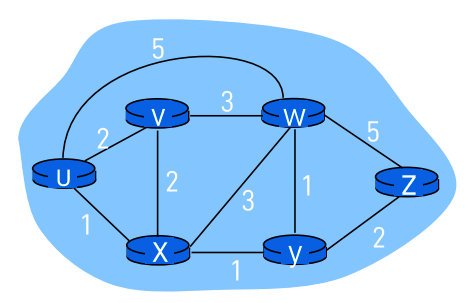
\includegraphics[width=0.39\textwidth]{rete-come-grafo.png}
    \caption{Rete come grafo}
\end{figure}\noindent
Un'altra informazione che ci interessa considerare è il costo di ogni collegamento
e di ogni percorso. Il costo di un collegamento è definito in base alla seguente
funzione $c$:
\[c:N\times N\to\mathbb{N}\]
Ad esempio, nella figura precedente $c(U,W)=5$. Di nuovo, il costo può essere
definito sulla base di parametri diversi: il numero di salti, la \emph{banda} o
l'inverso della \emph{banda} del link, la \emph{congestione}, ecc. Algoritmi
diversi possono usare parametri diversi.

\begin{note}
    Un costo definito sulla banda di un link è proporzionale al costo monetario
    di quel collegamento, mentre una definizione basata sull'inverso della banda
    è proporzionale al tempo di attraversamento.
\end{note}\noindent
Il costo di un percorso è espresso dalla funzione $cost$:
\[cost:\begin{array}[t]{ccl}
    N\times\dots\times N & \to & \mathbb{N}\\
    (n_1,\,\dots,\,n_k) & \mapsto & \sum_{i=1}^k c(n_1,\,n_2)
\end{array}\]
Ad esempio, $cost(U,X,Y,Z)=c(U,X)+c(X,Y)+c(Y,Z)=1+1+2=4$.

\subsection{Tipi di algoritmi di routing}
Gli algoritmi di routing si dividono in base al modo in cui sono distribuite le
informazioni sulla rete o in base al modo in cui sono configurate le tabelle di
routing.

\paragraph{Informazioni globali e distribuite}
Gli algoritmi basati su informazioni globali partono dall'ipotesi che ogni
\emph{router} abbia le stesse informazioni sulla tipologia della rete e i costi
dei collegamenti. D'altra parte, nel caso di informazioni distribuite, ogni
\emph{router} conosce solo i propri vicini e scambiando informazioni con essi
riesce a ricostruire i percorsi migliori. La prima tipologia di algoritmi è
detta essere a \quotes{\emph{link state}},cmentre la seconda a
\quotes{\emph{distance vector}}.

\paragraph{Configurazione statica e dinamica}
Le tabelle configurate staticamente sono definite manualmente
dall'amministratore di rete e rimangono invariate a meno di ulteriori interventi.
In questo caso non vengono neanche usati algoritmi di routing che infatti sono
necessari solo nel caso di tabelle generate dinamicamente.

\section{Algoritmo di Dijkstra}
L'algoritmo di Dijkstra è un algoritmo \emph{link state} quindi suppone che ogni
\emph{router} conosca la topologia della rete e il costo dei collegamenti.
Queste informazioni vengono fatte circolare mediante l'invio in broadcast di
messaggi.

La tabella di inoltro viene costruita eseguendo più volte l'algoritmo e, ad ogni
esecuzione, viene scoperto il percorso di costo minimo verso una destinazione.
Di conseguenza, eseguendo $k$ volte l'algoritmo, si ottengono i percorsi a costo
minimo verso $k$ destinazioni.

Prima di vedere la logica di funzionamento dell'algoritmo è necessario introdurre
della notazione specifica:
\begin{itemize}
    \item $D(v)$: definisce il costo del percorso verso il \emph{router} $v$;
    \item $p(v)$: definisce il predecessore del \emph{router} $v$ nel cammino
    verso esso;
    \item $N'$: insieme dei \emph{router} per i quali è già stato calcolato il
    cammino di costo minimo;
\end{itemize}
\begin{note}
    Il costo $c(n_1,n_2)$ del collegamento tra $n_1$ e $n_2$ vale $\infty$ se
    questi non solo collegati.
\end{note}

\begin{minicode}{Implementazine algoritmo di Dijkstra}
\com{Inizializzazione}
\rmbreak N' = \{u\}\hfill\com{$N'$ è inizialmente pari al nodo corrente}
foreach (v $\in$ N) do\\
    \indf if (v $\in$ u.adj()) then\\
        D(v) = c(u, v)\\
    \indf else\\
        D(v) = $\infty$\\
\rmbreak\com{Loop}
do\\
    \indf\bc{NODE} w = min(N - N')\hfill\com{Trova $w$ non ancora in $N'$ tale che D(w) sia minimo}
    \indf N'.insert(w)\hfill\com{Aggiunge $w$ a $N'$}
    \indf foreach (v $\in$ w.adj() - N')\hfill\com{Per ogni nodo $v$ adiacente a $w$ che non è in $N'$}
        \indff if (D(w) + c(w, v) < D(v)) then\\
            D(v) = D(w) + c(w, v)\hfill\com{Aggiorna il costo del percorso verso v}
            p(v) = w\hfill\com{Aggiorna il predecessore di $v$}
\rmbreak while (N'.size() < N.size())\hfill\com{Finché non sono stati inseriti tutti i nodi}
\end{minicode}\noindent
In sintesi, per ogni nodo $v$, se il costo che si paga per arrivare a $w$ e
superare il collegamento da $w$ a $v$ è minore del costo che attualmente si paga
per arrivare a $v$, allora il percorso minimo verso $v$ diventa il percorso passante
per $w$. In caso contrario, il percorso già noto per arrivare a $v$, è migliore
di quello che si avrebbe passando per $w$.

\begin{figure}[h!]
    \centering
    \subfloat[Passi di costruzione della tabella di routing con \emph{Dijkstra}]{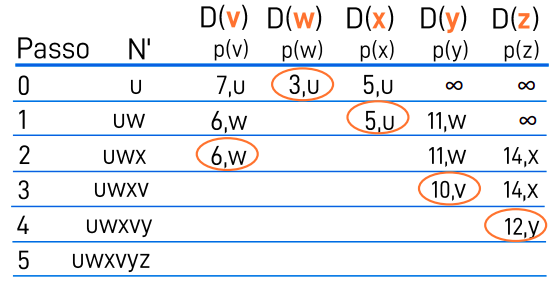
\includegraphics[width=0.56\textwidth]{tabella-dijkstra1.png}}
    \hfill
    \subfloat[Grafo di una rete]{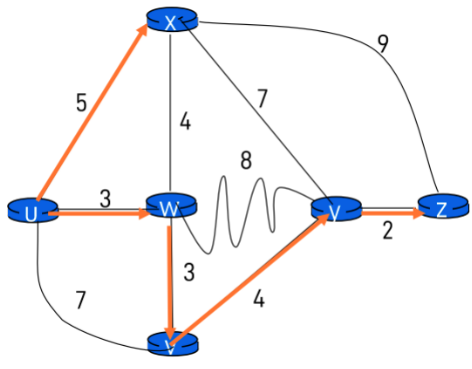
\includegraphics[width=0.4\textwidth]{grafo-rete1.png}}
    \caption{Esecuzione dell'algoritmo di \emph{Dijkstra}}
\end{figure}

\begin{note}
    Questo algoritmo costruisce i percorsi minimi partendo dal \emph{router} di
    destinazione e procedendo a ritroso sui predecessori.
\end{note}
\begin{note}
    Nel caso risultassero più percorsi minimi dal costo uguale se ne sceglie uno
    arbitrariamente.
\end{note}

\newpage\noindent
La tabella di inoltro risultante è la seguente:
\begin{figure}[ht]
    \centering
    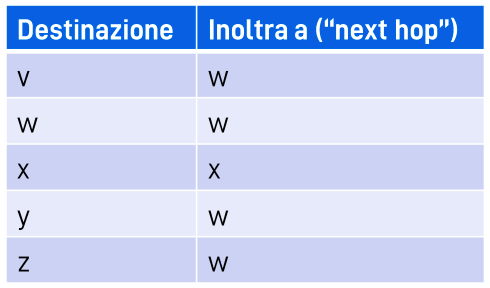
\includegraphics[width=0.48\textwidth]{tabella-dijkstra1-ris.png}
    \caption{Tabella di inoltro risultante}
\end{figure}

\subsection{Complessità e problemi dell'algoritmo}
In una rete con $n$ nodi (\emph{router}) vengono controllati tutti i nodi
$w\notin N'$ e quindi vengono eseguiti $\frac{n(n-1)}{2}=O(n^2)$ confronti.
Esistono tuttavia implementazioni più efficienti che portano la complessità a
$O(n\log n)$.

Il problema dell'algoritmo di \emph{Dijkstra} è che se i costi sono definiti male
l'algoritmo potrebbe oscillare. Ad esempio, se i costi sono definiti come la
quantità di traffico trasportata dai collegamenti, vale:

\begin{figure}[h!]
    \centering
    \subfloat[Situazione iniziale: $C$ genera un traffico di $e$ byte, $D$ e $B$ di $1$ byte]
    {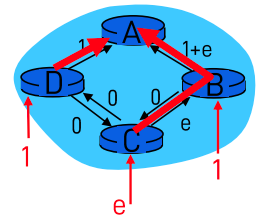
\includegraphics[width=0.35\textwidth]{problema-dijkstra1.png}}
    \hspace{3cm}
    \subfloat[Dati i nuovi costi, $Dijkstra$ calcola nuovi percorsi generando costi diversi]
    {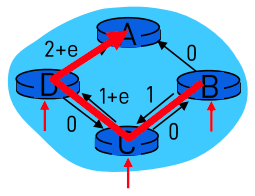
\includegraphics[width=0.35\textwidth]{problema-dijkstra2.png}}\\
    \subfloat[Nuovamente, dati i nuovi costi, $Dijkstra$ calcola altri nuovi percorsi generando costi diversi]
    {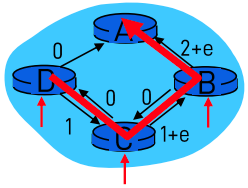
\includegraphics[width=0.35\textwidth]{problema-dijkstra3.png}}
    \hspace{3cm}
    \subfloat[Di nuovo ancora, dati i nuovi costi, $Dijkstra$ calcola altri nuovi percorsi generando costi diversi]
    {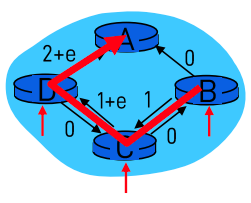
\includegraphics[width=0.35\textwidth]{problema-dijkstra4.png}}
    \caption{Esempio di oscillazione dell'algoritmo di \emph{Dijkstra}}
\end{figure}

\section{Protocollo OSPF}
\subsection{Autonomous system}
La rete internet è organizzata in moltissime sottoreti ognuna delle quali è di
proprietà di una qualche entità più o meno grande (e.g. \emph{\gls{glos:ISP}},
operatori di rete, aziende, \dots). Idealmente, ciascuna di queste sottoreti è
amministrativamente autonoma, ovvero configurabile liberamente dall'amministratore,
e capace di collegarsi alle altre sottoreti.
Queste caratteristiche hanno permesso la suddivisione di internet in
\emph{\gls{glos:AS}}:
\begin{definition}[AS - Autonomous System]
    Un autonomous system è un gruppo di router appartenenti ad uno stesso
    controllo amministrativo e identificato univocamente da un numero\footnotemark.
\end{definition}
\footnotetext{I numeri identificativi sono assegnati centralmente dai registri
regionali dell'\emph{\gls{glos:ICANN}}}\noindent
Questa suddivisione permette di scomporre il problema della generazione delle
tabelle di inoltro in due sotto problemi: gestire il routing all'interno di un
\emph{AS} e tra \emph{AS} diversi. A questo punto è lecito parlare di
\emph{Intra-AS routing} e \emph{Inter-AS routing}.

\bigskip\noindent
Nel contesto dell'\emph{Intra-AS routing} è stato introdotto il protocollo
\emph{\gls{prot:OSPF}}, un protocollo di tipo \emph{link state} e che si serve
dell'algoritmo di \emph{Dijkstra} per il calcolo dei percorsi.

Una particolarità di questo protocollo è che non si serve del \emph{livello di
trasporto} per consegnare i \emph{pacchetti}, bensì sfrutta l'indirizzo
\emph{multicast} $224.0.0.5$.

\subsection{Funzionamento del protocollo}
L'\emph{OSPF} è un protocollo molto semplice e infatti si compone soltanto di
tre procedure:
\begin{enumerate}
    \item \emph{Protocollo di \quotes{Hello}}: è una procedura che gestisce lo
    scambio di messaggi di mantenimento che servono a testare i collegamenti per
    vedere quali sono ancora attivi e quindi capire anche quali tra i
    \emph{router} adiacenti sono ancora raggiungibili;
    \item \emph{Protocollo di \quotes{Exchange}}: viene usato per comunicare ai
    \emph{router} adiacenti con i quali si è appena entrati in contatto la
    topologia conosciuta della rete;
    \item \emph{Protocollo di \quotes{Flooding}}: viene usato per informare
    tutti i \emph{router} di un cambiamento avvenuto nello stato dei collegamenti;
\end{enumerate}
In particolare, la procedura di \emph{flooding} prevede che un \emph{router}
trasmetta su tutte le sue interfacce un messaggio e che tutti gli altri
\emph{router} facciano lo stesso. Ovviamente, quando ciò avviene, il messaggio
non viene ritrasmesso dall'interfaccia che l'ha ricevuto. Questa procedura viene
detta essere di \emph{flooding controllato} e comporta che vengano inviati tanti
messaggi quanti sono i collegamenti o i \emph{domini di broadcast}.

\subsection{OSPF gerarchico}
In reti con molti \emph{router}, per ridurre il numero di messaggi inviati, si
divide la rete in modo gerarchico. La gerarchia che si va a costituire ha due
livelli: una dorsale, o \emph{backbone}, e le reti di area.

In questo modo, i messaggi circolano solo all'interno delle reti di area e
i \emph{router} conoscono solo la topologia della propria area e il cammino
più breve verso le altre. Nello specifico, sono solo i \emph{router di
bordo} di ogni area a conoscere le informazioni relative alle rotte verso le
reti interne alla propria area. Queste sono le informazioni che l'\emph{OSPF}
comunica a tutti gli altri \emph{router di bordo} delle altre aree.

A sua volta, anche la dorsale è un'area a se stante e i \emph{router} al suo
interno comunicano mediante \emph{OSPF}.

\begin{figure}[h!]
    \centering
    \subfloat[8 messaggi inviati]{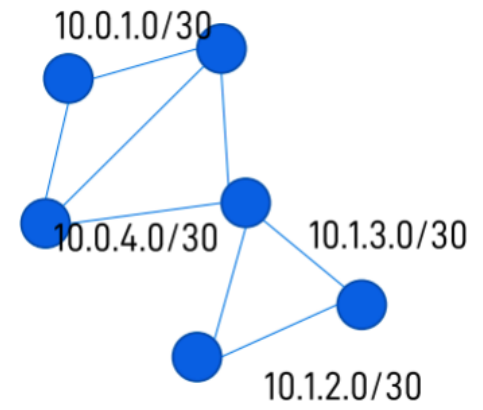
\includegraphics[width=0.48\textwidth]{rete-ospf1.png}}
    \hfill
    \subfloat[2 messaggi inviati]{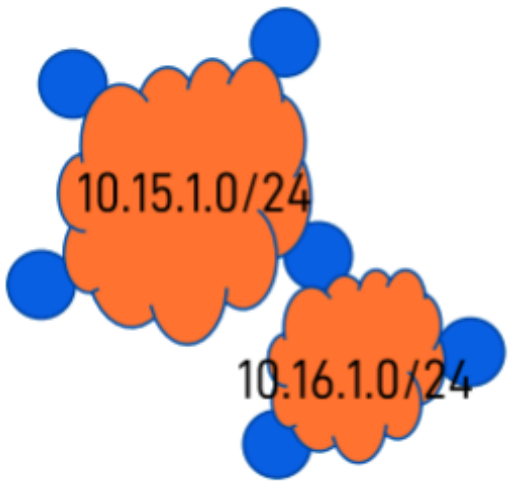
\includegraphics[width=0.48\textwidth]{rete-ospf2.png}}\\
    \subfloat[I messaggi circolano solo all'interno delle reti di area]{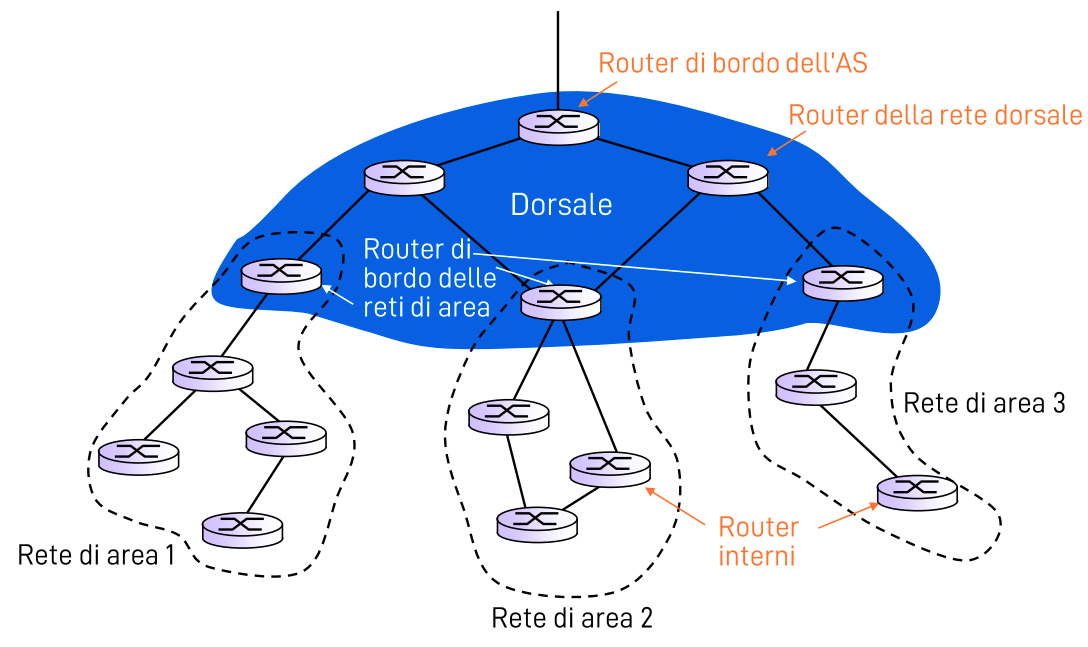
\includegraphics[width=0.75\textwidth]{ospf-gerarchico.png}}
\end{figure}

\subsection{Traffic engineering}
Poiché l'\emph{OSPF} è un protocollo \emph{link state} nel quale l'unica cosa che
influenza la scelta di un percorso è il costo dei collegamenti. Gli amministratori
di un \emph{AS} potrebbero \quotes{modificare} il costo di alcuni collegamenti in
modo da indurre il protocollo a indirizzare il traffico verso quelle rotte.

Questa possibilità inverte le relazioni di causa-effetto del protocollo, ovvero,
dato un obiettivo di \emph{traffic engineering} è possibile agire sul costo di
un collegamento per raggiungere quell'obiettivo.

\section{Algoritmo di Bellman-Ford}
Il \emph{Bellman-Ford} è un algoritmo di tipo \emph{distance vector} e quindi
parte dall'ipotesi che ogni \emph{router} sappia soltanto quali \emph{router} gli
sono vicini e quanto costa raggiungerli. La conoscenza della rete perciò, non è
globale, ma distribuita e ogni \emph{router} scambia informazioni con i propri
vicini per capire come raggiungere reti più distanti.

\subsection{Logica di funzionamento}
Introduciamo la seguente notazione:
\begin{itemize}
    \item $N_x$: è l'insieme dei vicini del \emph{router} $x$;
    \item $R_x$: è la tabella di inoltro del \emph{router} $x$:
    \begin{itemize}
        \item $R_x[d]$: è la riga della tabella relativa alla destinazione $d$:
        \begin{itemize}
            \item $R_x[d].cost$: costo per raggiungere $d$;
            \item $R_x[d].nexthop$: indirizzo di \emph{next hop};
            \item $R_x[d].time$: riferimento temporale al momento in cui il percorso
            è stato impostato;
        \end{itemize}
    \end{itemize}
    \item $D_x$: \emph{distance vector} del \emph{router} $x$, ovvero il vettore
    contente tutte le destinazioni raggiungibili da $x$ e i relativi costi;
\end{itemize}
\begin{note}
    I costi dei collegamenti sono anche detti distanze o metriche.
\end{note}
\begin{note}
    Viene salvato l'istante di scoperta di un percorso in modo che quelli troppo
    vecchi possano essere scartati.
\end{note}

\begin{minicode}{Implementazione algoritmo Bellman-Ford}
\com{Inizializzazione}
\par\noindent\rmbreak\ind foreach (n $\in$ $N_x$) do\hfill\com{Per tutti i vicini $n$ di $x$}
    $R_x$[n].cost = c(x,n)\hfill\com{Imposta il costo per raggiungere $n$}
    $R_x$[n].nexthop = n\hfill\com{Imposta $n$ come \emph{next hop}}
    $R_x$[n].time = now()\\
\nl\rmbreak\com{Ogni $T$ secondi}
\rmbreak $\langle$\bc{NODE}, int$\rangle$ $D_x$ = new $\langle$\bc{NODE}, int$\rangle$[$R_x$.size()]\hfill\com{\emph{Distance vector} di $x$}
\par\noindent\rmbreak\ind foreach (d $\in$ $R_x$) do\hfill\com{Per tutte le destinazioni $d$ conosciute da $x$}
    $D_x$[d] = $\langle$d, $R_x$[d].cost$\rangle$\hfill\com{Popola il \emph{distance vector}}
\par\noindent\rmbreak\ind foreach (n $\in$ $N_x$) do\hfill\com{Per tutti i vicini $n$ di $x$}
    send($D_x$, n)\hfill\com{Invia il \emph{distance vector}}
\nl\rmbreak\com{Quando si riceve il \emph{distance vector} $D_y$ di un vicino $y$}
\par\noindent\rmbreak\ind foreach ($\langle$d, cost$\rangle$ $\in$ $D_y$) do\hfill\com{Per ogni coppia destinazione-costo del vettore}
    \indf if (d $\notin$ $R_x$ or cost + c(x, y) < $R_x$[d] or y == $R_x$[d].nexthop) then\\
        $R_x$.cost = cost + c(x, y)\hfill\com{Imposta il costo per raggiungere la $d$}
        $R_x$.nexthop = y\hfill\com{Imposta il \emph{next hop}}
        $R_x$.time = now()\hfill\com{Imposta il tempo di scoperta}
\end{minicode}

\newpage
\begin{eg}[Esempio di esecuzione dell'algoritmo Bellman-Ford]
Inizialmente ogni router conosce solo le rotte che lo collegano
direttamente ai propri vicini.

\begin{figure}[h!]
    \centering
    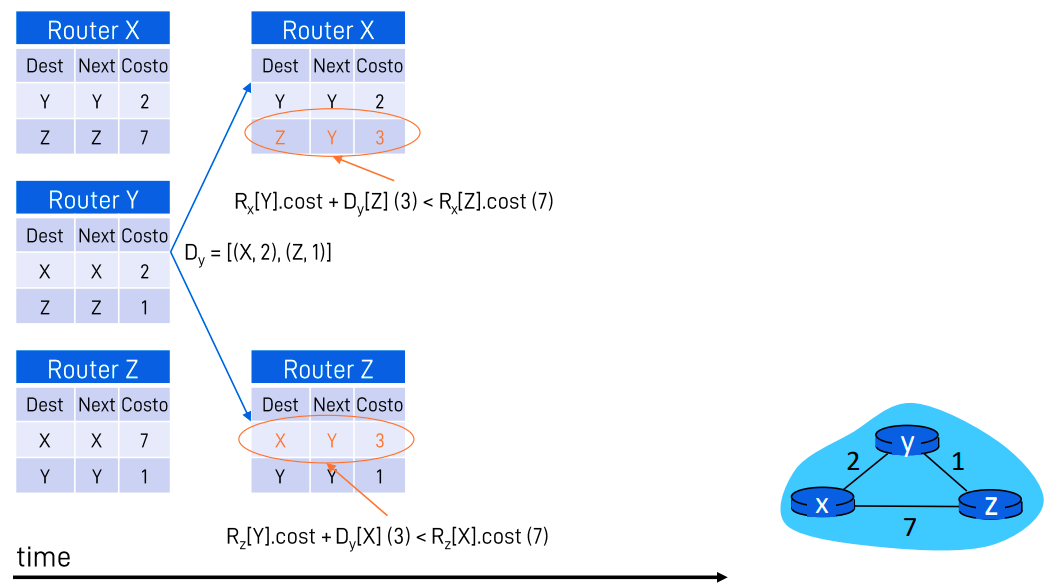
\includegraphics[width=0.9\textwidth]{bellman1.png}
    \caption{$Y$ trasmette il proprio \emph{distance vector}}
\end{figure}\noindent
Dopo che $Y$ ha trasmesso il proprio distance vector, $X$ e $Z$
confrontano le rotte ricevute con quelle che hanno già. Poiché il collegamento
tra $X$ e $Z$ costa 7, mentre passando per $Y$ si ottiene un cammino di costo 3,
$X$ e $Z$ aggiornano le proprie tabelle modificando rispettivamente le rotte
verso $Z$ e verso $X$, sostituendole con un nuovo percorso passante per $Y$.

\begin{figure}[h!]
    \centering
    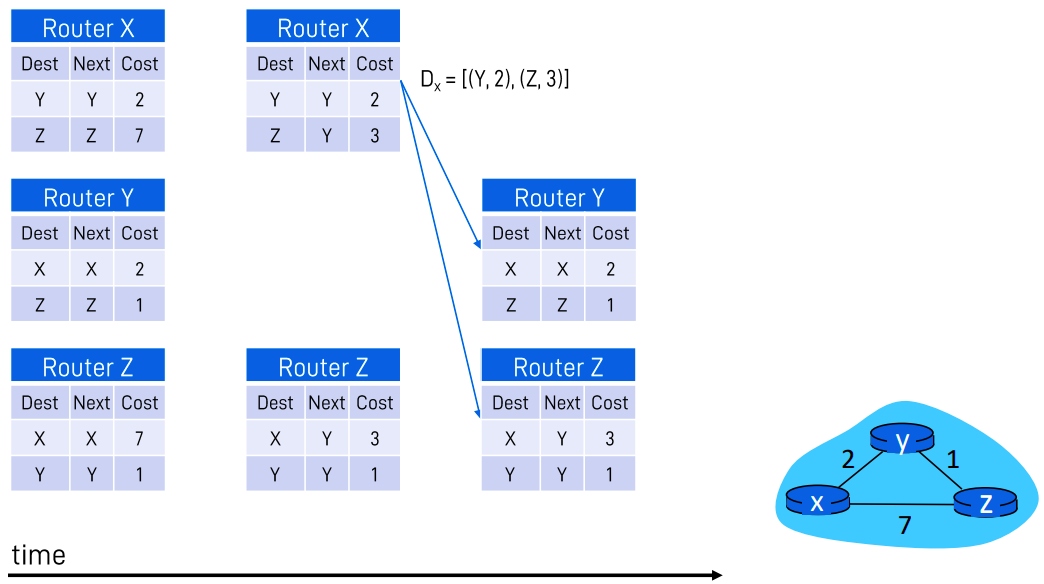
\includegraphics[width=0.9\textwidth]{bellman2.png}
    \caption{$X$ trasmette il proprio \emph{distance vector}}
\end{figure}\noindent
Dopo che $X$ ha trasmesso il proprio distance vector, né $Y$, né $Z$ hanno
necessità di aggiornare le proprie tabelle in quanto non scoprono destinazioni
nuove e nemmeno percorsi migliori per le destinazioni già conosciute.

\begin{figure}[ht!]
    \centering
    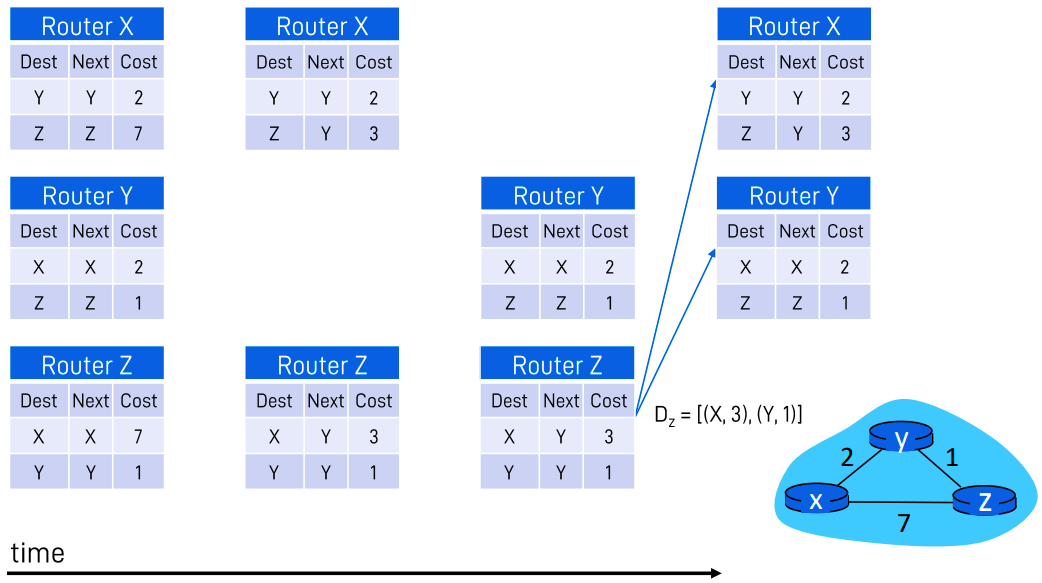
\includegraphics[width=0.9\textwidth]{bellman3.png}
    \caption{$Z$ trasmette il proprio \emph{distance vector}}
\end{figure}\noindent
Infine, $Z$ trasmette il proprio distance vector, ma anche in questo
caso non c'è necessità di aggiornare le tabelle. A questo punto, tutti i router
della rete sanno come raggiungersi nel modo più economico possibile.
\end{eg}

\subsection{Problema del count-to-infinity}
Il problema del \emph{count-to-infinity} si verifica quando cade un collegamento
di uno dei cammini brevi. Gli \emph{host} che utilizzavano quel collegamento e che non
sono ad esso direttamente collegati, non vengono informati del suo cambiamento
di stato e quindi continuano ad inoltrare \emph{pacchetti} attraverso quel percorso.
Quando però il \emph{router} collegato a quel link deve decidere dove inoltrare i
\emph{pacchetti}, sapendo di non poter usare quel collegamento, li ritrasmette
al mittente. Il mittente a quel punto, aggiorna il costo di quel percorso e,
se rimane il più conveniente, riprova ad utilizzarlo. Questo scambio continua
fino a quando il percorso fallace risulta più conveniente di altri
percorsi \quotes{sani}. Quando finalmente il percorso difettoso risulterà non
più conveniente, i \emph{router} ne sceglieranno uno diverso.

\begin{eg}[Problema del count-to-infinity]
Si consideri la seguente configurazione di rete:

\begin{figure}[h!]
    \centering
    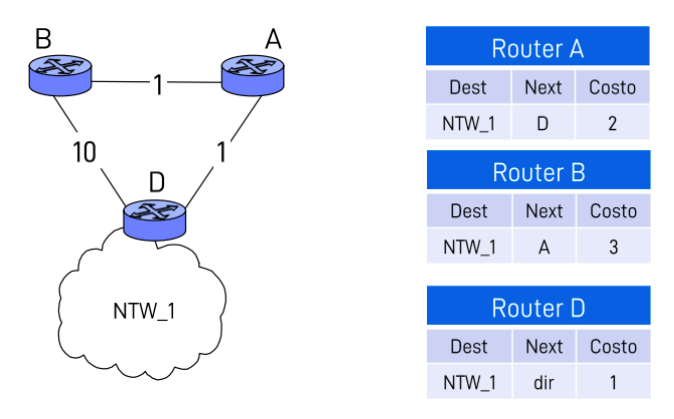
\includegraphics[width=0.5\textwidth]{count-to-infinity1.png}
\end{figure}\noindent
Supponiamo che il collegamento di costo 1 tra $A$ e $D$ si rompa. Se $B$ deve
inviare un pacchetto alla rete \texttt{NTW\_1}, lo inoltra verso il
router $A$. Non sapendo a chi inviarlo, $A$ lo ritrasmette a $B$.

\begin{figure}[ht!]
    \centering
    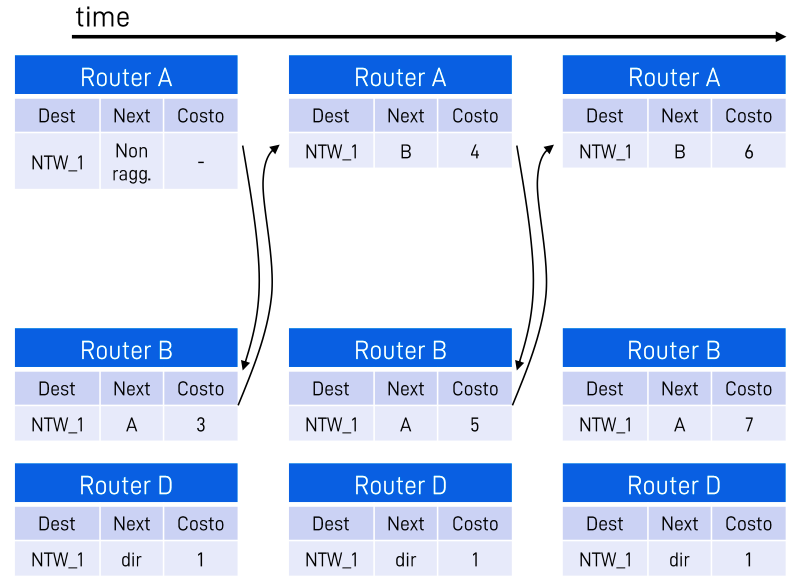
\includegraphics[width=0.9\textwidth]{count-to-infinity2.png}
    \caption{Loop del \emph{count-to-infinity}}
\end{figure}\noindent
Dopo molti scambi, il collegamento di costo 10 tra $B$ e $D$ risulterà più
conveniente di quello che passa per $A$ col risultato che $B$ smetterà di
reinoltrare il pacchetto ad $A$, rompendo il loop del count-to-infinity.
\begin{figure}[h!]
    \centering
    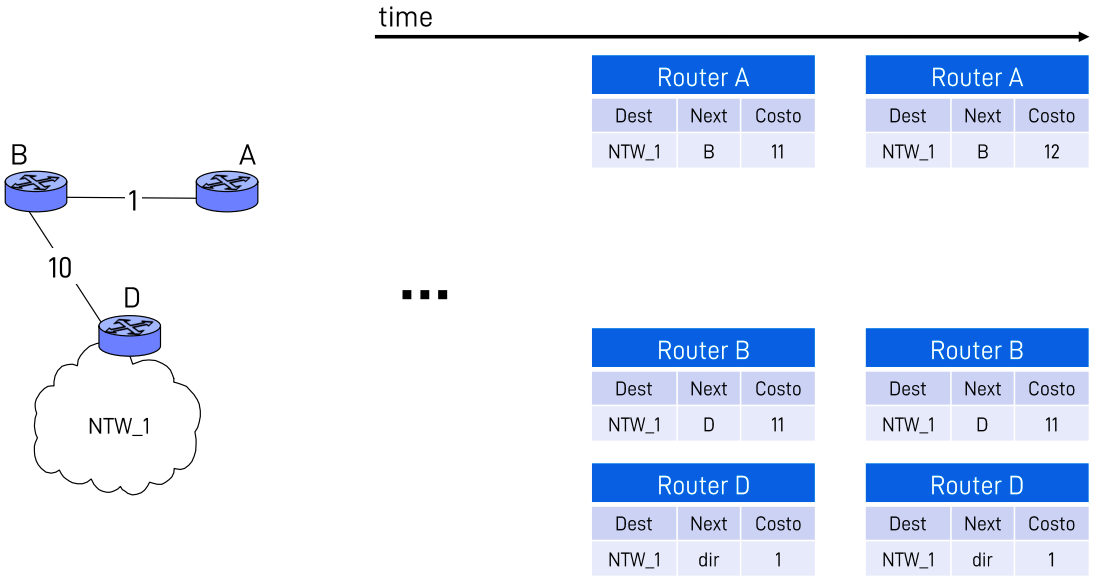
\includegraphics[width=0.9\textwidth]{count-to-infinity3.png}
    \caption{Termine del loop e aggiornamento dei cammini brevi}
\end{figure}
\end{eg}

\paragraph{Soluzioni al count-to-infinity}
Fortunatamente, esistono delle procedure che permettono di evitare l'insorgere
di questo problema:
\begin{itemize}
    \item \emph{Limite al numero di hop}: viene impostato un limite al numero di
    \emph{hop} (tipicamente 15) dei \emph{pacchetti} che trasportano i
    \emph{distance vector}. Questo permette di ridurre il tempo di convergenza;
    \item \emph{Split horizon}: quando un \emph{router} manda ad un vicino
    aggiornamenti al costo dei percorsi, omette quelli appresi da quello stesso
    vicino;
    \item \emph{Poisoned reverse}: dati tre \emph{router} $X$, $Y$ e $Z$, fino
    a quando $X$ raggiunge $Z$ passando per $Y$, $X$ comunica ad $Y$ che $D_x(Z)=\infty$;
\end{itemize}
\begin{note}
    Nell'esempio precedente, con lo \emph{split horizon}, $B$ non avrebbe incluso
    la riga \texttt{(NTW\_1, 3)} nel proprio \emph{distance vector} perché l'aveva
    appresa proprio da $A$.
\end{note}
\begin{note}
    Sempre nell'esempio precedente, se fosse stato utilizzato il \emph{poisoned
    reverse}, $B$ avrebbe incluso la riga \texttt{(NTW\_1, $\infty$)} nel
    \emph{distance vector} inviato ad $A$ perché $B$ raggiunge \texttt{NTW\_1}
    passando per $A$. Questa riga avrebbe portato $A$ a scegliere di non inoltrare
    di nuovo il \emph{pacchetto} a $B$.
\end{note}\noindent
In generale possiamo affermare che le informazioni relative a miglioramenti nei
costi dei cammini si propagano molto più velocemente rispetto alle informazioni
sul peggioramento dei costi.

Purtroppo però, le procedure di \emph{split horizon} e \emph{poisoned reverse}
non funzionano sempre, ma sono influenzate dall'ordine di invio dei \emph{distance
vector}. Infatti, poiché i \emph{router} agiscono in modo indipendente tra loro,
non è noto a priori l'ordine di invio dei \emph{distance vector} e questo può
portare allo sviluppo di cicli.

\begin{eg}[Esempio di generazione di cicli con split horizon]
Si prenda la seguente configurazione di rete:

\begin{figure}[h!]
    \centering
    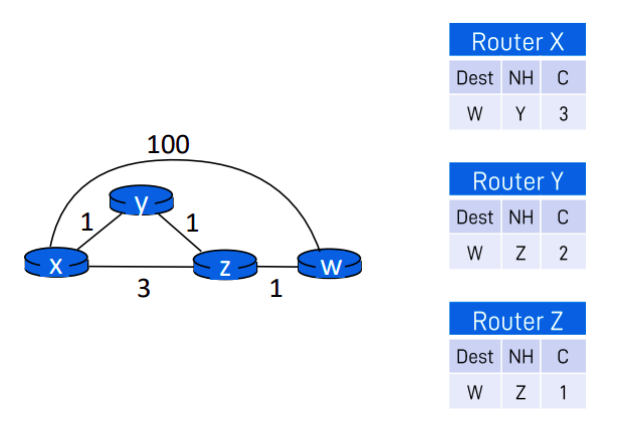
\includegraphics[width=0.6\textwidth]{split-horizon1.png}
\end{figure}\noindent
Supponiamo che il collegamento tra $Z$ e $W$ si rompa. Se adesso $X$ trasmette
a $Y$ e $Z$ il proprio distance vector, utilizzando la procedura di
split horizon, si viene a creare un ciclo.
\newpage
\begin{figure}[ht!]
    \centering
    \subfloat{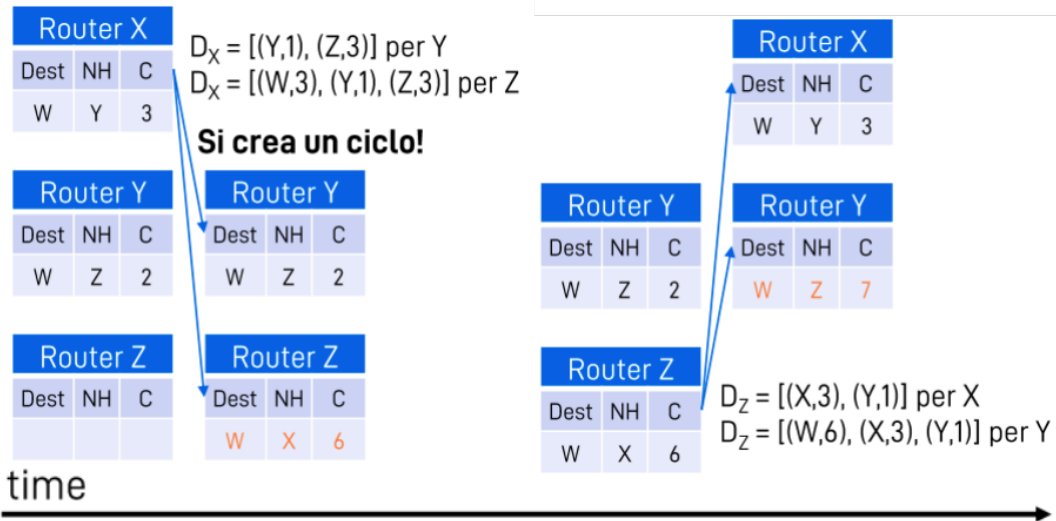
\includegraphics[width=0.6\textwidth]{split-horizon2.png}}
    \\
    \subfloat{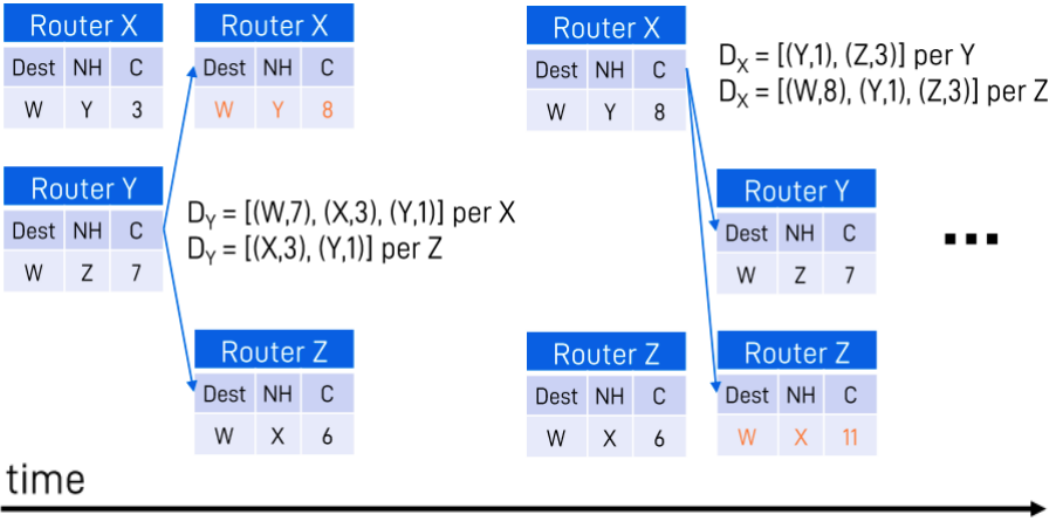
\includegraphics[width=0.6\textwidth]{split-horizon3.png}}
    \caption{Sviluppo del ciclo}
\end{figure}\noindent
Alla fine, il collegamento tra $X$ e $W$ di costo 100 risulterà conveniente
e, quindi, $X$ propagherà quell'informazione a tutti i suoi vicini terminando il
ciclo.

\begin{figure}[h!]
    \centering
    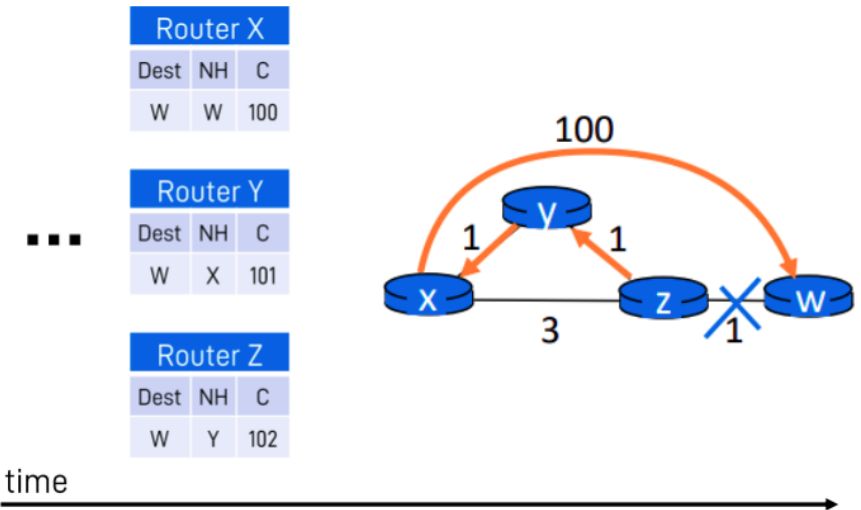
\includegraphics[width=0.6\textwidth]{split-horizon4.png}
    \caption{Fine del ciclo}
\end{figure}
\end{eg}

\section{Protocollo RIP}
Il \emph{\gls{prot:RIP}} è un protocollo per il \emph{routing intra-AS}, cioè
interno a un \emph{Autonomous System} ed è Implementato utilizzando i
\emph{distance vector}. Il \emph{RIP} è un protocollo semplice da implementare e
gestire, ma è adatto solo a reti con una dimensione ridotta e comunque la
convergenza è abbastanza lenta.

Il principio di funzionamento è molto semplice: ogni 30 secondi, o quando cambiano
le tabelle di routing, il \emph{RIP} trasmette, sulla porta 520 e
all'\emph{indirizzo multicast} $224.0.0.9$, un messaggio di \emph{RIP advertisement}.
Questo messaggio contiene un elenco che comprende fino a 25 sottoreti di
destinazione all'interno dell'\emph{AS} e la distanza del mittente rispetto a
ciascuna sottorete.

Nel \emph{RIP}, il costo di un percorso è dato dal numero di \emph{hop} necessari
ad attraversarlo e per limitare il tempo di convergenza viene impostato un limite
di 15 \emph{hop} e vengono considerati di costo infinito i percorsi che ne
richiedono 16 o più. È comunque possibile che un \emph{hop} abbia un costo più
che unitario.

\begin{note}
    Il \emph{RIP} si serve di \emph{\gls{prot:UDP}} per trasportare i messaggi.
\end{note}

\begin{eg}[Esempio di funzionamento del RIP]
Si considerino la seguente rete e la tabella di inoltro del router $D$:
\begin{figure}[h!]
    \centering
    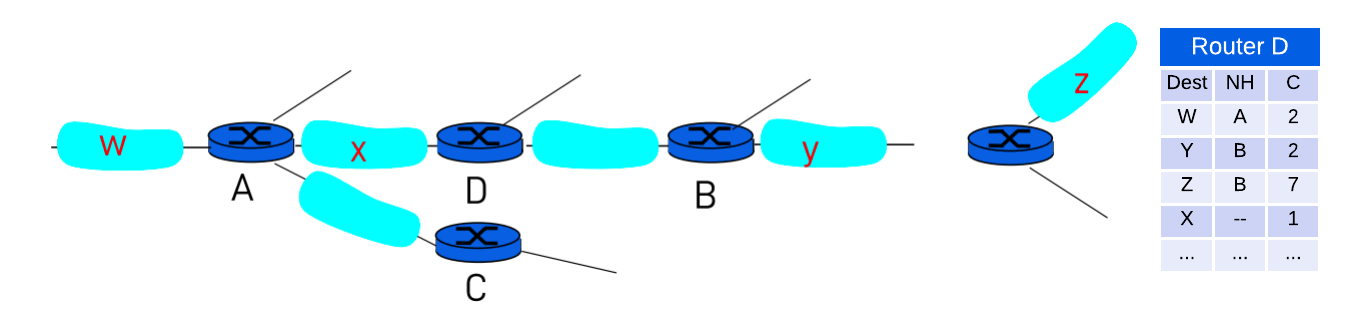
\includegraphics[width=\textwidth]{rip1.png}
\end{figure}

\noindent
Dopo che $A$ ha trasmesso il proprio RIP advertisement, $D$ può modificare la
propria rotta verso la sottorete $Z$ impostando quella passante per $A$ che ha
un costo minore.

\begin{figure}[h!]
    \centering
    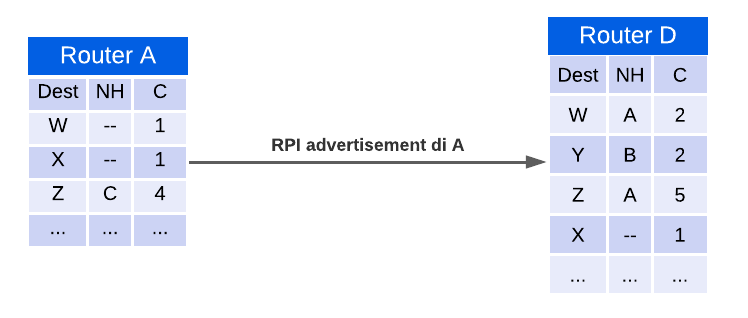
\includegraphics[width=0.8\textwidth]{rip2.png}
    \caption{Adattamento della tabella di inoltro}
\end{figure}
\end{eg}

\paragraph{Gestione dei guasti}
Se un \emph{router} non riceve notizie da un suo vicino per 3 minuti, quel vicino
e il collegamento con esso vengono considerati guasti. Di conseguenza, il
\emph{router} modifica la propria tabella di instradamento locale e propaga
l'informazione a tutti gli altri \emph{router} adiacenti. Se il \emph{RIP
advertisement} porta i vicini a modificare le proprie tabelle di inoltro, quei
\emph{router} trasmettono a loro volta i propri \emph{RIP advertisement} così da
diffondere l'informazione su tutta la rete. Viene usata la tecnica del
\emph{poisoned reverse} per evitare loop.

\paragraph{Gestione delle tabelle di inoltro}
Come accennato in precedenza, il \emph{RIP} è implementato come un protocollo di
\emph{livello Applicativo} e quindi usa una \emph{socket} come interfaccia di
trasmissione e ricezione. In realtà però, il protocollo \emph{RIP} viene eseguito
da un processo chiamato \texttt{routed} che mantiene le informazioni di
instradamento e scambia i messaggi con i vicini.

\section{Confronto tra algoritmi link state e distance vector}
Negli algoritmi di tipo \emph{link state} i messaggi vengono inviati ad ogni
\emph{router} e attraverso ogni collegamento, quindi se $n$ è il numero di
\emph{router} ed $E$ il numero di collegamenti, il numero di messaggi inviati è
$O(nE)$. D'altra parte, gli algoritmi a \emph{distance vector} comunicano solo
con i propri vicini, ma come abbiamo visto, i costi dipendono dall'organizzazione
della rete.

Per quanto riguarda i tempi di convergenza invece, gli algoritmi a \emph{link
state} sono soggetti a oscillazioni, mentre quelli a \emph{distance vector}
soffrono del problema del \emph{count-to-infinity} e potrebbero generare cicli.

Infine, relativamente al comportamento in caso di guasti, con algoritmi
\emph{link state} i \emph{router} gestiscono la propria tabella in modo
indipendente, ma potrebbero trasmettere informazioni sbagliate sui costi.
Anche utilizzando i \emph{distance vector} i \emph{router} potrebbero comunque
comunicare costi sbagliati e poiché la tabella di ogni \emph{router} è usata
anche dagli altri, gli errori si propagherebbero attraverso la rete.

\section{Protocollo BGP}
Il \emph{\gls{prot:BGP}} è un protocollo per la comunicazione \emph{Inter-AS} che
costituisce lo standard de facto nella comunicazione in internet.
Prima di vederne nel dettaglio il funzionamento però, è bene ritornare sul
concetto di \emph{\hyperref[def:17]{AS}}.

\bigskip\noindent
Gli \emph{AS} comunicano tra loro per condividere informazioni di raggiungibilità,
ma ogni \emph{AS} può decidere in autonomia quali sono i suoi punti di ingresso
e di uscita e anche quali informazioni condividere con ciascun vicino.

Esistono anche \emph{AS} particolari che non condividono informazioni proprie,
ma fungono semplicemente da tramite per altri \emph{AS}.

\subsection{Principi di funzionamento}
\emph{BGP} è un protocollo del \emph{livello Applicativo} e infatti utilizza il
\emph{\gls{prot:TCP}} per connettere coppie di \emph{nodi} detti \emph{BGP
speaker}. Tra due \emph{BGP speaker} possono esistere più connessioni
contemporaneamente.

\paragraph{Protocollo path vector}
Il \emph{BGP} è un protocollo di tipo \emph{path vector} e ciò significa che
oltre alle informazioni di raggiungibilità di una rete comunica anche il
percorso che usa per raggiungerla.
Ad esempio, un \emph{path vector} è qualcosa come la seguente:
\begin{figure}[h!]
    \centering
    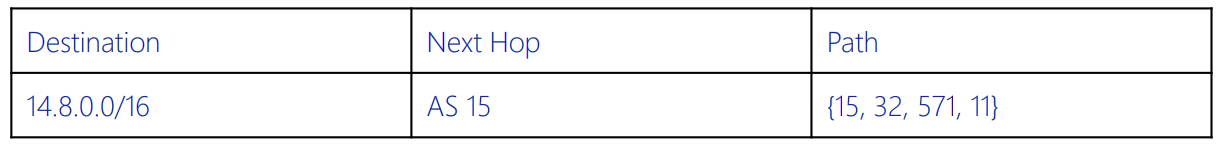
\includegraphics[width=\textwidth]{path-vector.png}
    \caption{Esempio di \emph{path vector}}
\end{figure}

\noindent
L'idea alla base del \emph{BGP} infatti, è che un \emph{nodo} non condivida solo
l'informazione su quali destinazioni può raggiungere, ma anche il percorso che
utilizza.

In particolare, grazie a \emph{BGP}, un \emph{AS} in qualsiasi momento può
condividere e ritirare le informazioni di raggiungibilità verso una o alcune
delle proprie reti interne.

\newpage
\paragraph{Macchina a stati del BGP}
Il funzionamento del \emph{BGP} può essere descritto da una macchina a stati:

\begin{figure}[h!]
    \centering
    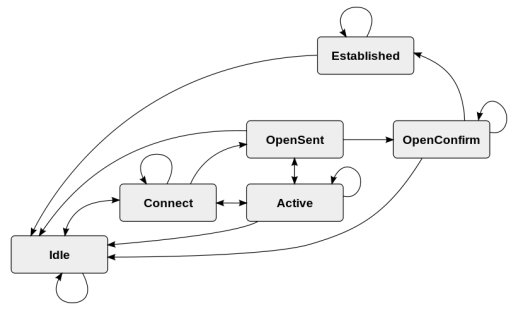
\includegraphics[width=\textwidth]{bgp-stati.png}
    \caption{Macchina a stati del \emph{BGP}}
\end{figure}

\paragraph{Interconnessioni e policy}
Esistono tre tipi di connessioni tra \emph{AS}:
\begin{itemize}
    \item \emph{Client-Provider}: il client paga il provider per essere
    raggiungibile;
    \item \emph{Provider-Client}: il provider viene pagato per garantire la
    raggiungibilità di un client;
    \item \emph{Peer}: due nodi sono peer quando condividono tra loro le
    rispettive informazioni di raggiungibilità;
\end{itemize}
Nello specifico, le interconnessioni sono regolate da contratti o \emph{policy}
che stabiliscono quali informazioni possono essere condivise con un certo 
vicino e quali no. Esistono due tipi di \emph{policy}:
\begin{itemize}
    \item \emph{Ingress policies}: stabiliscono quali informazioni possono entrare
    all'interno dell'\emph{AS};
    \item \emph{Egress policies}: stabiliscono quali informazioni possono uscire
    dall'\emph{AS};
\end{itemize}

\paragraph{Best path BGP}
Il concetto di \emph{best path} nel \emph{BGP}, o percorso migliore, è diverso
da quello del routing classico. Nel routing classico si cerca il percorso più
breve o meno costoso, nel \emph{BGP} invece, non c'è un parametro generale, ma
dipende dal singolo \emph{AS}.

\begin{figure}[ht]
    \centering
    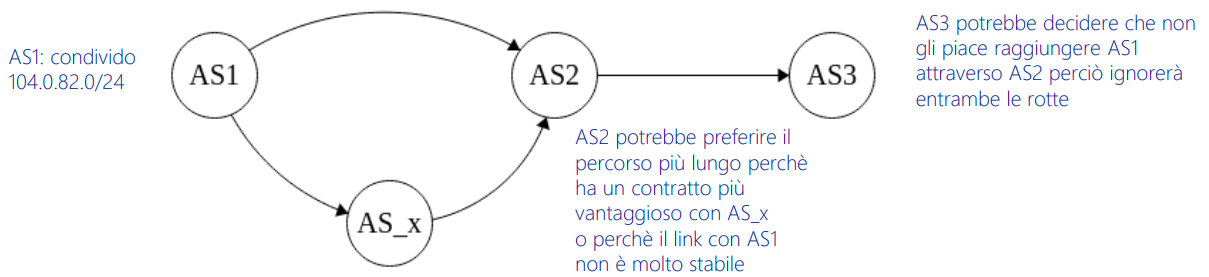
\includegraphics[width=\textwidth]{bgp-best-path.png}
    \caption{Esempio di \emph{best path BGP}}
\end{figure}

\newpage\noindent
Comunque, quando due \emph{BGP speaker} si scambiano tra loro le informazioni di
raggiungibilità per le destinazioni, condividono soltanto i \emph{best path}
verso quelle destinazioni. Ovviamente, se un \emph{nodo} decide di non voler
attraversare certi \emph{AS}, i percorsi che li includono non verranno mai
considerati \emph{best path} da quel \emph{nodo} e quindi non verranno neanche
condivisi.

\begin{note}
    Il \emph{best path} potrebbe non essere il percorso più veloce.
\end{note}

\subsection{Messaggi BGP}
Il protocollo \emph{BGP} usa un sistema di messaggistica basata su quattro tipi
di messaggi: \texttt{Open}, \texttt{Notification}, \texttt{KeepAlive} e
\texttt{Update}.

\paragraph{Messaggio Open}
L'\texttt{Open} è un messaggio usato per aprire una connessione \emph{BGP}.
Se il messaggio viene accettato il destinatario risponde con un messaggio di
tipo \texttt{KeepAlive} e soltanto a quel punto la connessione verrà considerata
aperta.

\begin{figure}[h!]
    \centering
    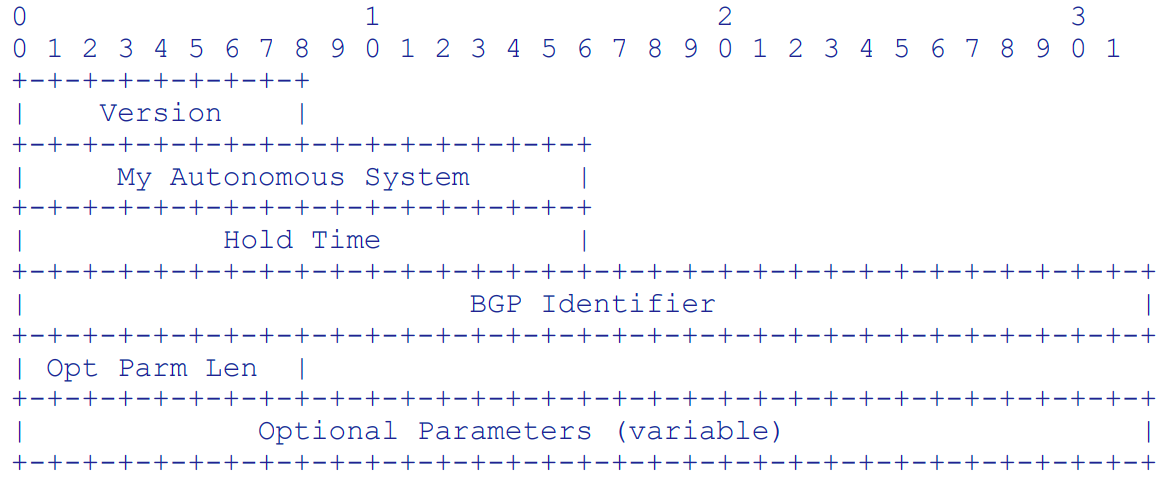
\includegraphics[width=\textwidth]{bgp-open-msg.png}
    \caption{Struttura di un messaggio di tipo \texttt{Open}}
\end{figure}\noindent
Il campo \texttt{Hold Time} indica per quanto tempo mantenere aperta la
connessione. Ognuno dei due \emph{BGP speaker} propone un \texttt{Hold Time} e
viene scelto il minore. Il campo \texttt{BGP Identifier} contiene
l'\emph{indirizzo IP} identificativo dello \emph{speaker} ed è uguale per
tutte le sue interfacce.

\newpage
\paragraph{Messaggio Notification}
Questo messaggio serve soltanto a informare un \emph{BGP speaker} del verificarsi
di un errore.

\begin{figure}[h!]
    \centering
    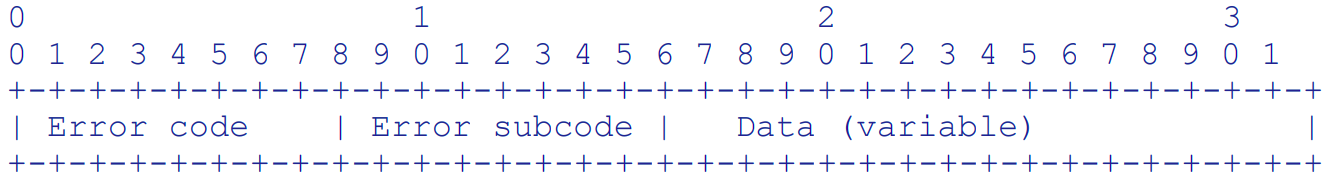
\includegraphics[width=\textwidth]{bgp-notification-msg.png}
    \caption{Struttura di un messaggio di tipo \texttt{Notification}}
\end{figure}

\paragraph{Messaggio KeepAlive}
Lo scopo dei messaggi di \texttt{KeepAlive} è impedire lo scadere
dell'\texttt{Hold Time} di una connessione. Possono anche essere inviati per
chiudere una connessione indicando un \texttt{Hold Time} di 0 secondi.
Per non congestionare la rete, questi messaggi consistono soltanto di un
header \emph{BGP} di 19 byte senza ulteriori contenuti.

\paragraph{Messaggi Update}
Gli \texttt{Update} contengono le informazioni di raggiungibilità e gli
attributi correlati e sono i messaggi responsabili per la diffusione delle
informazioni. In particolare, le informazioni trasportate possono essere di due
tipi:
\begin{itemize}
    \item \emph{Additive}: trasportano informazioni relative a nuovi percorsi;
    \item \emph{Sottrattive}: rimuovono dei percorsi esistenti;
\end{itemize}
L'azione di rimozione di una rotta è detta \emph{withdraw} e fa uso di una
specifica sezione dei messaggi \emph{BGP} nella quale vengono indicate le rotte
da cancellare. I \emph{withdraw} vengono usati quando una destinazione non è
più raggiungibile attraverso nessun percorso.

\begin{figure}[h!]
    \centering
    \subfloat[Situazione iniziale]{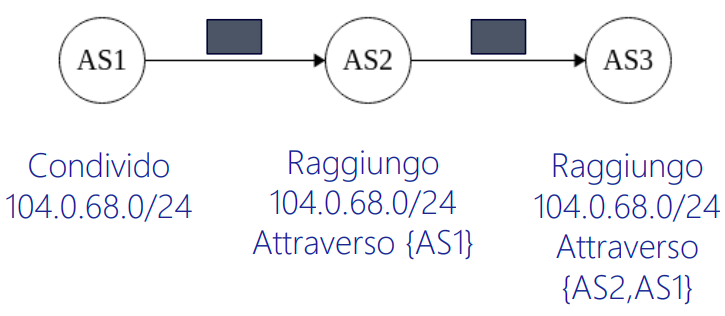
\includegraphics[width=0.61\textwidth]{bgp-withdraw1.png}}
    \hfill
    \subfloat[Rimozione della rotta]{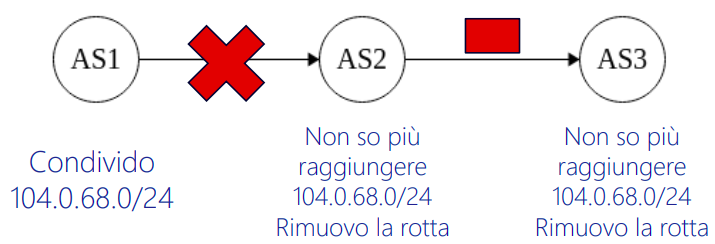
\includegraphics[width=0.61\textwidth]{bgp-withdraw2.png}}
    \caption{Utilizzo dei messaggi di \texttt{Update} con \emph{withdraw}}
\end{figure}

\noindent
Quando un \emph{AS} apprende una rotta migliore per una destinazione per
condividere l'informazione con i suoi vicini può trasmettere un \texttt{Update}
con il \emph{withdraw} della rotta precedente e un secondo \texttt{Update} con
la rotta nuova.

\begin{figure}[ht]
    \centering
    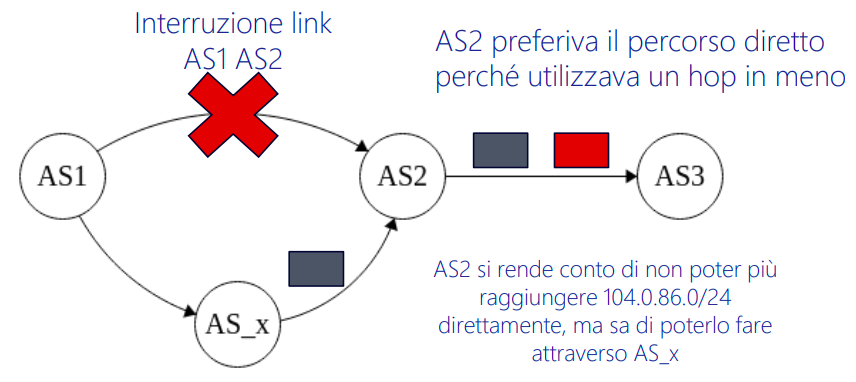
\includegraphics[width=0.8\textwidth]{bgp-update-withdraw.png}
    \caption{Aggiornamento di una rotta}
\end{figure}

\noindent
Ciò può essere fatto anche con un solo messaggio usando il \emph{withdraw implicito}.
\begin{figure}[h!]
    \centering
    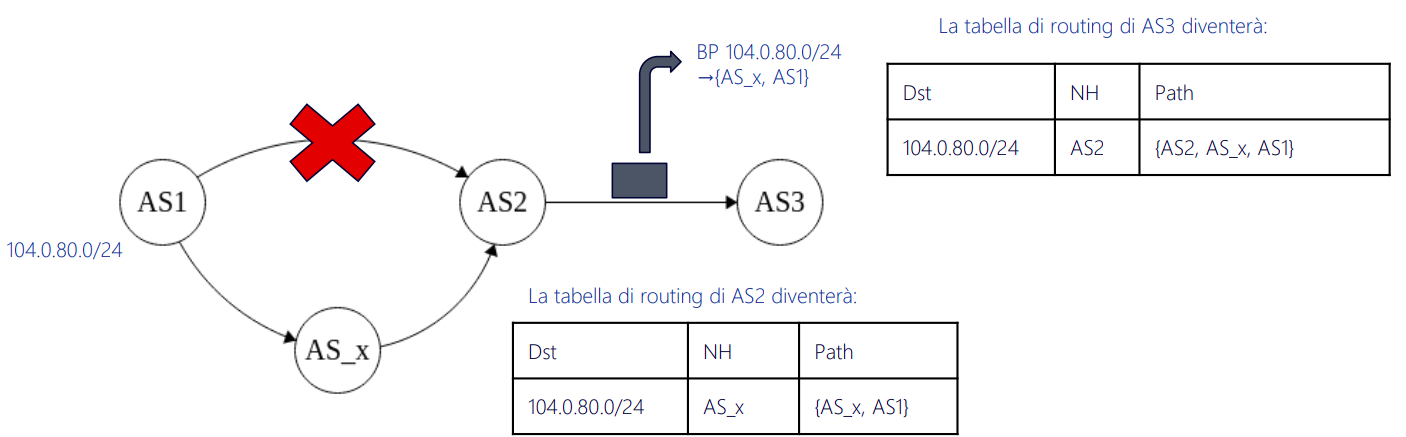
\includegraphics[width=\textwidth]{bgp-withdraw-implicito.png}
    \caption{Aggiornamento di una rotta con \emph{withdraw implicito}}
\end{figure}

\subsection{Gestione delle rotte}
Per poter risparmiare informazioni all’interno dei \emph{pacchetti}, generalmente,
le rotte vengono aggregate pagando una perdita di precisione nel percorso.

\begin{figure}[h!]
    \centering
    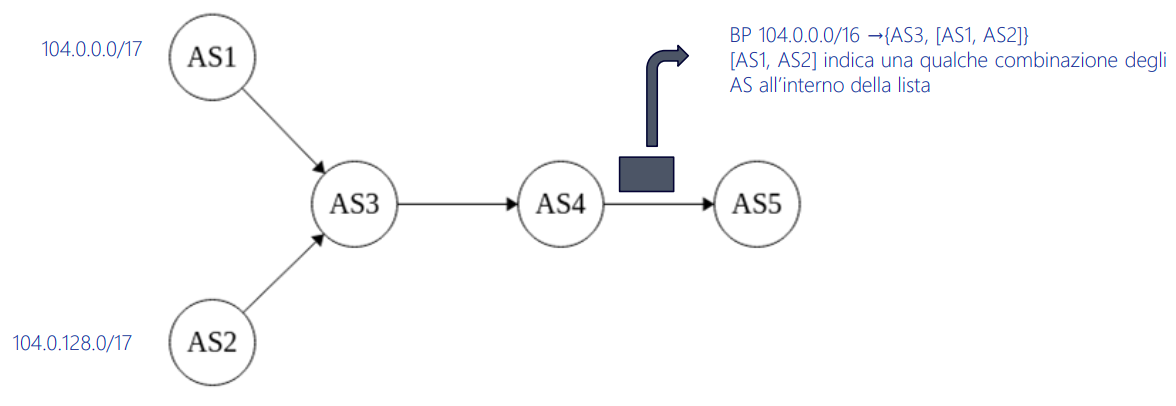
\includegraphics[width=\textwidth]{bgp-aggregazione-rotte.png}
    \caption{Aggregazione delle rotte}
\end{figure}

\paragraph{Filtri}
I filtri controllano ciò che entra e ciò che esce da un \emph{AS} e a seconda dei
casi si parla di \emph{ingress filters} e \emph{egress filters}. È possibile
definire filtri specifici per ogni connessione e possono essere generici
(e.g. non lasciar passare nulla che contenga $AS19$) o molto precisi (e.g. si
può arrivare ad analizzare i singoli \emph{frame}). Ovviamente, tutti i
\emph{pacchetti} che non superano i filtri vengono scartati.

\paragraph{Routing Information Base - RIB}
Il \emph{BGP} utilizza tre tabelle per gestire le rotte:
\begin{itemize}
    \item \texttt{ADJ\_RIB\_IN}: contiene le rotte che sono state accettate in
    ingresso e che verranno valutate per ricercare percorsi alternativi;
    \item \texttt{Routing table}: contiene i \emph{best path} attuali;
    \item \texttt{ADJ\_RIB\_OUT}: contiene le rotte che hanno superato i filtri
    in uscita e che devono essere condivise
\end{itemize}
Quando viene ricevuto un messaggio di \texttt{Update}, se il \emph{pacchetto}
supera i filtri in ingresso, viene modificata la tabella \texttt{ADJ\_RIB\_IN}
e in particolare, se il messaggio trasporta una nuova rotta, questa viene aggiunta
alla tabella, se invece si tratta di un \texttt{Update} con \emph{withdraw}, la
rotta viene rimossa. A quel punto, viene rivalutato il \emph{best path} per la
rotta aggiornata e, se è migliore di quello attuale, oppure consente di raggiungere
una nuova destinazione, vengono aggiornate anche la \texttt{Routing table} e la
tabella \texttt{ADJ\_RIB\_OUT}. I nuovi cambiamenti vengono infine trasmessi
a tutti gli altri vicini.